\documentclass[8pt]{article}
\usepackage[a4paper,landscape,margin=1in]{geometry}
\usepackage{cmbright}

\usepackage{amsmath}
\usepackage{nicefrac}
\usepackage{siunitx}

\usepackage{array}
\usepackage{booktabs}
\usepackage{longtable}

\usepackage{xcolor}
\definecolor{urlblue}{HTML}{0000ee}
\usepackage{hyperref}
\hypersetup{%
colorlinks = true,%
urlcolor   = urlblue,%
}

\usepackage{tcolorbox}
\usepackage{varwidth}

\setlength\parindent{0pt}
\pagenumbering{gobble}

\begin{document}
\begin{figure}[!ht]
% MF group logo
\begin{minipage}[b][2.5cm][c]{.72\textwidth}
\href{http://foroozandeh.chem.ox.ac.uk/home}%
{\includegraphics[scale=1.8]{/home/simon/Documents/DPhil/projects/spectral_estimation/NMR-EsPy/nmrespy/images/mf_logo.png}}
\end{minipage}
% NMR-EsPy logo
\begin{minipage}[b][2.5cm][c]{.27\textwidth}
\href{https://foroozandehgroup.github.io/NMR-EsPy}%
{\includegraphics[scale=0.5]{/home/simon/Documents/DPhil/projects/spectral_estimation/NMR-EsPy/nmrespy/images/nmrespy_full.png}}
\end{minipage}
\end{figure}

\texttt{15:11:03\\02-10-2021}

% user provided description
\subsection*{Description}
Gramicidin \textsuperscript{1}H data, region: 4.92 - 4.63Hz. NLP result.

% experiment parameters
\subsection*{Experiment Information}
\hspace{-6pt}
\begin{longtable}[l]{c c}
\toprule
Parameter & F1
\\\midrule
Transmitter frequency (MHz) & 699.85349925\\
Sweep width (Hz) & 213.3550492785903\\
Sweep width (ppm) & 0.30485673002597374\\
Transmitter offset (Hz) & 3341.8042558034504\\
Transmitter offset (ppm) & 4.775005425256435\\
\bottomrule
\end{longtable}

% estimation result
\subsection*{Result}
\begin{longtable}[l]{c c c c c c c c}
\toprule
$m$ & $a_m$ & $\phi_m\ (\text{rad})$ & $f_m\ (\text{Hz})$ & $f_m\ (\text{ppm})$ & $\eta_m\ (\text{s}^{-1})$ & $\int$ & $\nicefrac{\int}{\left\lVert\int\right\rVert}$\\
\midrule
1 & 0.97993 & \num{4.0324e-3} & \num{3.2871e+3} & 4.6969 & 8.2264 & 650.16 & \num{6.0447e-3}\\
- & $\pm$0.1278 & $\pm$\num{4.449e-3} & $\pm$0.16563 & $\pm$\num{2.3666e-4} & $\pm$1.4632 & - & -\\
2 & 2.3856 & \num{3.7641e-3} & \num{3.2936e+3} & 4.7061 & 13.561 & \num{1.5828e+3} & \num{1.4715e-2}\\
- & $\pm$0.45776 & $\pm$\num{6.4395e-3} & $\pm$0.26776 & $\pm$\num{3.826e-4} & $\pm$1.9138 & - & -\\
3 & 3.044 & \num{3.6958e-3} & \num{3.296e+3} & 4.7095 & 10.4 & \num{2.0196e+3} & \num{1.8777e-2}\\
- & $\pm$0.48547 & $\pm$\num{7.713e-3} & $\pm$0.14453 & $\pm$\num{2.0652e-4} & $\pm$1.1678 & - & -\\
4 & 4.325 & \num{3.1198e-3} & \num{3.3021e+3} & 4.7182 & 13.091 & \num{2.8695e+3} & \num{2.6678e-2}\\
- & $\pm$0.45296 & $\pm$\num{2.1621e-2} & $\pm$0.12842 & $\pm$\num{1.8349e-4} & $\pm$1.1173 & - & -\\
5 & 1.4544 & \num{2.8389e-3} & \num{3.3048e+3} & 4.7222 & 10.626 & 964.98 & \num{8.9716e-3}\\
- & $\pm$0.36242 & $\pm$\num{1.2439e-2} & $\pm$0.2602 & $\pm$\num{3.718e-4} & $\pm$1.9003 & - & -\\
6 & 0.66128 & \num{2.67e-3} & \num{3.3104e+3} & 4.7301 & 9.157 & 438.75 & \num{4.0791e-3}\\
- & $\pm$0.10934 & $\pm$\num{5.515e-3} & $\pm$0.18101 & $\pm$\num{2.5864e-4} & $\pm$4.237 & - & -\\
7 & 34.354 & \num{2.8139e-2} & \num{3.3219e+3} & 4.7466 & 10.417 & \num{2.2785e+4} & 0.21183\\
- & $\pm$0.3352 & $\pm$\num{4.6813e-3} & $\pm$\num{5.2083e-3} & $\pm$\num{7.442e-6} & $\pm$\num{8.8721e-2} & - & -\\
8 & 38.49 & \num{7.8199e-3} & \num{3.3276e+3} & 4.7547 & 13.392 & \num{2.5537e+4} & 0.23742\\
- & $\pm$1.3742 & $\pm$\num{1.003e-2} & $\pm$\num{2.4113e-2} & $\pm$\num{3.4454e-5} & $\pm$0.23202 & - & -\\
9 & 96.49 & \num{1.0098e-2} & \num{3.3308e+3} & 4.7592 & 14.521 & \num{6.4016e+4} & 0.59517\\
- & $\pm$1.776 & $\pm$\num{1.1853e-2} & $\pm$\num{1.6274e-2} & $\pm$\num{2.3254e-5} & $\pm$0.15523 & - & -\\
10 & 76.126 & \num{-2.3636e-3} & \num{3.3365e+3} & 4.7675 & 12.877 & \num{5.0508e+4} & 0.46959\\
- & $\pm$2.415 & $\pm$\num{1.2294e-2} & $\pm$\num{1.6893e-2} & $\pm$\num{2.4138e-5} & $\pm$0.19536 & - & -\\
11 & 73.317 & \num{-4.2277e-3} & \num{3.3396e+3} & 4.7718 & 16.224 & \num{4.8644e+4} & 0.45225\\
- & $\pm$2.332 & $\pm$\num{1.34e-2} & $\pm$\num{2.5507e-2} & $\pm$\num{3.6447e-5} & $\pm$0.27129 & - & -\\
12 & 46.883 & \num{-8.731e-3} & \num{3.3455e+3} & 4.7803 & 12.701 & \num{3.1105e+4} & 0.28919\\
- & $\pm$0.97279 & $\pm$\num{7.1597e-3} & $\pm$\num{1.2994e-2} & $\pm$\num{1.8566e-5} & $\pm$0.17045 & - & -\\
13 & 28.115 & \num{-5.899e-3} & \num{3.35e+3} & 4.7868 & 27.356 & \num{1.8653e+4} & 0.17342\\
- & $\pm$1.4184 & $\pm$\num{7.0406e-3} & $\pm$0.10111 & $\pm$\num{1.4448e-4} & $\pm$0.97513 & - & -\\
14 & 10.694 & \num{-2.1451e-3} & \num{3.3585e+3} & 4.7989 & 23.14 & \num{7.0951e+3} & \num{6.5964e-2}\\
- & $\pm$0.57579 & $\pm$\num{5.5494e-3} & $\pm$\num{9.1491e-2} & $\pm$\num{1.3073e-4} & $\pm$0.99546 & - & -\\
15 & 0.69935 & \num{2.4271e-3} & \num{3.3664e+3} & 4.8102 & 21.516 & 463.99 & \num{4.3138e-3}\\
- & $\pm$0.17306 & $\pm$\num{4.2503e-3} & $\pm$0.57553 & $\pm$\num{8.2236e-4} & $\pm$2.9804 & - & -\\
16 & 0.11889 & \num{2.9417e-3} & \num{3.4047e+3} & 4.8649 & 7.4464 & 78.879 & \num{7.3335e-4}\\
- & $\pm$\num{8.3761e-2} & $\pm$\num{6.4565e-3} & $\pm$1.0829 & $\pm$\num{1.5474e-3} & $\pm$8.146 & - & -\\
\bottomrule
\end{longtable}

% figure of result
\begin{center}
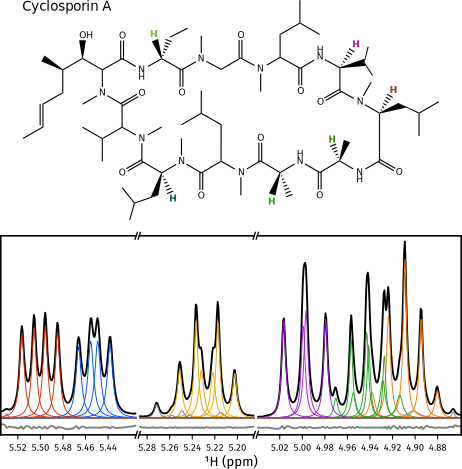
\includegraphics{/tmp/figure.pdf}
\end{center}

% blurb
\small
\begin{tcolorbox}[hbox]
\begin{varwidth}{\textwidth}
Estimation performed using \textsc{NMR-EsPy}.\\
Author: Simon Hulse\\
For more information:\\[5pt]
{\raisebox{-4pt}{\includegraphics[scale=0.029]{/home/simon/Documents/DPhil/projects/spectral_estimation/NMR-EsPy/nmrespy/images/book_icon.png}}}\hspace{1em}\href{https://foroozandehgroup.github.io/NMR-EsPy}{\texttt{https://foroozandehgroup.github.io/NMR-EsPy}}\\[5pt]
{\raisebox{-4pt}{\includegraphics[scale=0.12]{/home/simon/Documents/DPhil/projects/spectral_estimation/NMR-EsPy/nmrespy/images/github.png}}}\hspace{1em}\href{https://github.com/foroozandehgroup/NMR-EsPy}{\texttt{https://github.com/foroozandehgroup/NMR-EsPy}}\\[5pt]
{\raisebox{-3pt}{\includegraphics[scale=0.015]{/home/simon/Documents/DPhil/projects/spectral_estimation/NMR-EsPy/nmrespy/images/email_icon.png}}}\hspace{1em}\href{mailto:simon.hulse@chem.ox.ac.uk?subject=NMR-EsPy query}{\texttt{simon.hulse@chem.ox.ac.uk}}\\[5pt]
If used in a publication, please cite:\\
\textit{No references yet...}
\end{varwidth}
\end{tcolorbox}

\end{document}
